\chapter{Sonnenfelsplatz i byen Graz i Østrig kontra Nytorv/Østerågade i byen Aalborg i Danmark}
\label{chap:sonnenfelsplatz_i_byen_Graz_i_ostrig kontra_nytorv/osteraagade_i_byen_aalborg_i_danmark}

Den Østrigske by Graz renoverede i 2011 Sonnenfelsplatz til et Shared Space område. Sonnenfelsplatz er en central plads som har butikker og restauranter. Derudover ligger byens universitet campus lige i nærheden. \autocite{ssing2015}
I belastningsperioder har Sonnenfelsplatz i byen Graz i Østrig 15.000 køretøjer, 3.400 fodgængere og 640 cyklister i timen. I følge anvendelsen af Shared Space, anbefaler de at Shared Space bør anvendes ved trafikmængder på maks. 3.000- 4.000 motorkøretøjer/døgn, hvilket ikke er tilfældet i byen Graz i Østrig. \autocite{vejlednigomss2013}
Da køretøjerne skaber de fleste trafikbelastninger, og da vejoverfladen er skadet, og infrastrukturen under jorden har haft behov for renovering blev området lavet om. Herved blev Shared Space et mål for området, for at skabe en bebolig gade med frit kultur mobilitet, hvor der er plads til alle trafikanter. I den anledning er vejskilte og vejafmærkninger bevidst blevet valgt fra, da det vil få de forskellige trafikantgrupper til at integrere sig efter hinanden afhængigt af situationen i området. Dette kan også ses tydeligt på vejbanen.
På Sonnenfelsplatz er der ikke højdeforskel i vejen som afskiller kørertøjer fra fodgængere. Trafikanterne bliver opfordret til at dele og respekterer hinanden om pladsen. I midten af pladsen er der lavet en lille rundkørsel. Området anvender meget få skilte og vejmarkeringer, hvilket kan ses i området Sonnenfelsplatz, som ses på figur \cref{fig:cykelsti} på side \pageref{fig:cykelsti}. \autocite{SP2015}

\begin{figure}[htbp]
  \centering
  \begin{adjustbox}{max width=\textwidth}
    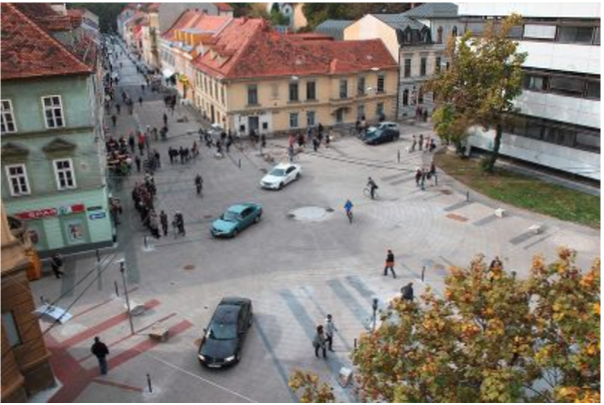
\includegraphics{figures/Billederogfigur/Perspektivering/en_andne_by.png}
 \end{adjustbox}
  \caption{Cykelsti \autocite{sonne}}
   \label{fig:cykelsti}
\end{figure}

~\\
I indledningen er Nytorv/Østerågade i byen Aalborg beskrevet som et samlingspunkt, hvor der på tilsvarende måde færdes mange mennesker og køretøjer. I området er der mange shopping- og cafémuligheder, derudover færdes der mange mennesker i området, som transportere sig med bus og på cykel. I følge trafiktællingerne der er foretaget i rapporten \cref{sub:trafiktaellinger} har Nytorv/Østerågade i byen Aalborg i Danmark et døgns trafik på 394 biler og der er 3.826 cykler på en november dag. I interviewet \cref{chap:interviews} mener flere af interviewpersoner, at bilerne og cyklisterne skaber utryghed for fodgængerne, hvilket giver årsag til, at der i rapporten fokuseres på at differentiere trafikantgrupperne. Det er blevet gjort ved at lave nogle forslag om at have en cykelbane i området, hvor cyklisterne kan cykle på deres egen bane, og en busluse for at udelukke bilerne fra området, hvilket kan ses på de nedenstående billeder.

~\\
Ligheden mellem området Sonnenfelsplatz i byen Graz og Nytorv/Østerågade i Aalborg er, at de to områder har nogle trafikantgrupper som deler kørerbanen. For Nytorvs/Østerågades tilfælde er der tale om fodgængere, cyklister, busser og erhvervsbiler for, og for Sonnenfelsplatz er det alle traffikantgrupperne der deler vejen.
~\\
Forskellen på de to områder er, at der er forbud for gennemkørsel af privatbiler på Nytorv/Østerågade, dog bliver færdselsloven ikke overholdt. Det er ikke tilfældet i Sonnenfelsplatz, da det er kørertøjerne der skaber de fleste trafikbelastninger. Ifølge døgns trafikken og blandt andet interviewpersonerne er det cyklisterne der skaber trafikbelastninger. Derudover bevæger området i Nytorv/Østerågade sig længere væk fra at være shared space og tættere på næsten at være en sivegade, da der blandt andet er højdeforskel i vejen som afskiller kørertøjer fra fodgængere. I Sonnenfelsplatz bevæger området sig tættere på at være Shared Space, da højdeforskellen på vejen ikke afskiller kørertøjer fra fodgængere.
